\documentclass[twocolumn]{miniclass}
\usepackage[utf8]{inputenc}
\usepackage[english]{babel}
\usepackage{caption}
\usepackage{subcaption}

\usepackage{blindtext}
\usepackage[none]{hyphenat}
\usepackage{float}

%\usepackage[switch]{lineno}  % Use for twocolumn environment
%\usepackage{lineno}  % Use for onecolumn environment
%\linenumbers

\title{Title of your work here}

\author[1,$\ast$]{Patryk Jarnot}
\affil[1]{Department of Computer Network and Systems, Silesian University of Technology}
\affil[$\ast$]{patryk.jarnot@polsl.pl}

\date{}

\begin{document}

\maketitle


\section{Introduction}
Lorem ipsum dolor sit amet, consectetur adipiscing elit. Morbi tincidunt odio nec risus vehicula, id accumsan odio elementum. Aliquam massa arcu, congue sit amet turpis ac, molestie ultrices ligula. Quisque iaculis non odio ut accumsan. Donec vitae risus quis nibh volutpat aliquam. Vivamus imperdiet sit amet ex at finibus. Morbi ornare pretium pharetra. Sed venenatis quis mi condimentum egestas. Nullam vitae tincidunt metus. Praesent venenatis lacinia sagittis. Praesent in ex auctor lacus porttitor dictum vel vitae nunc.

Aenean at euismod arcu, non varius metus. Nunc ornare luctus arcu, bibendum cursus nulla accumsan nec. Sed tempor elit sit amet ipsum bibendum, vehicula laoreet diam tempor. Maecenas odio tellus, egestas vitae sem eget, feugiat semper ipsum. Cras sit amet vestibulum dui, nec volutpat purus. Aliquam rutrum lectus et vehicula dignissim. Praesent venenatis id lacus et porttitor. Proin malesuada ligula a tincidunt cursus. Donec condimentum ultrices turpis, id maximus erat scelerisque at. Ut egestas viverra purus viverra ullamcorper. Vivamus cursus arcu elementum gravida fringilla. Maecenas odio ipsum, fringilla vel dui nec, egestas bibendum odio. Etiam semper sem id justo auctor pretium quis et mi.

\section{Methods}
Lorem ipsum dolor sit amet, consectetur adipiscing elit. Morbi tincidunt odio nec risus vehicula, id accumsan odio elementum. Aliquam massa arcu, congue sit amet turpis ac, molestie ultrices ligula. Quisque iaculis non odio ut accumsan. Donec vitae risus quis nibh volutpat aliquam. Vivamus imperdiet sit amet ex at finibus. Morbi ornare pretium pharetra. Sed venenatis quis mi condimentum egestas. Nullam vitae tincidunt metus. Praesent venenatis lacinia sagittis. Praesent in ex auctor lacus porttitor dictum vel vitae nunc Figure~\ref{fig:ann}.

\begin{figure}[H]
    \centering
    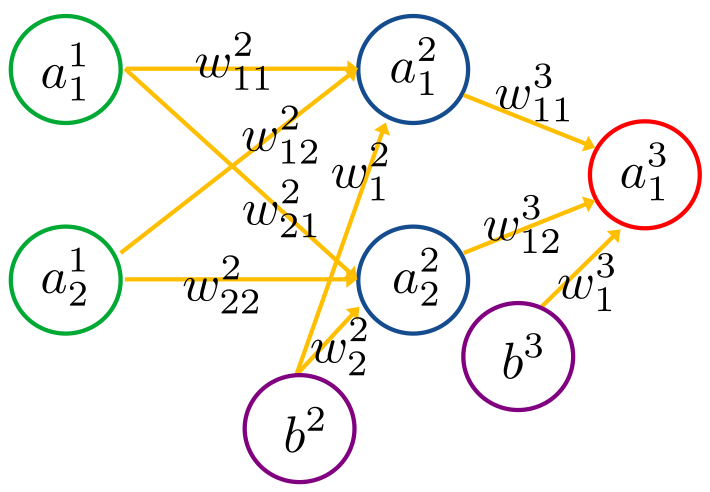
\includegraphics[width=230pt]{resources/ann.png}
    \caption{Awesome artificial neural network.}
    \label{fig:ann}
\end{figure}

\subsection{Subsection}
Lorem ipsum dolor sit amet, consectetur adipiscing elit. Morbi tincidunt odio nec risus vehicula, id accumsan odio elementum. Aliquam massa arcu, congue sit amet turpis ac, molestie ultrices ligula. Quisque iaculis non odio ut accumsan. Donec vitae risus quis nibh volutpat aliquam. Vivamus imperdiet sit amet ex at finibus. Morbi ornare pretium pharetra. Sed venenatis quis mi condimentum egestas. Nullam vitae tincidunt metus. Praesent venenatis lacinia sagittis. Praesent in ex auctor lacus porttitor dictum vel vitae nunc.

\subsubsection{Subsubsection}
Lorem ipsum dolor sit amet, consectetur adipiscing elit. Morbi tincidunt odio nec risus vehicula, id accumsan odio elementum. Aliquam massa arcu, congue sit amet turpis ac, molestie ultrices ligula. Quisque iaculis non odio ut accumsan. Donec vitae risus quis nibh volutpat aliquam. Vivamus imperdiet sit amet ex at finibus. Morbi ornare pretium pharetra. Sed venenatis quis mi condimentum egestas. Nullam vitae tincidunt metus. Praesent venenatis lacinia sagittis. Praesent in ex auctor lacus porttitor dictum vel vitae nunc.

\section{Results}
Lorem ipsum dolor sit amet, consectetur adipiscing elit. Morbi tincidunt odio nec risus vehicula, id accumsan odio elementum. Aliquam massa arcu, congue sit amet turpis ac, molestie ultrices ligula. Quisque iaculis non odio ut accumsan. Donec vitae risus quis nibh volutpat aliquam. Vivamus imperdiet sit amet ex at finibus. Morbi ornare pretium pharetra. Sed venenatis quis mi condimentum egestas. Nullam vitae tincidunt metus. Praesent venenatis lacinia sagittis. Praesent in ex auctor lacus porttitor dictum vel vitae nunc.

Aenean at euismod arcu, non varius metus. Nunc ornare luctus arcu, bibendum cursus nulla accumsan nec. Sed tempor elit sit amet ipsum bibendum, vehicula laoreet diam tempor. Maecenas odio tellus, egestas vitae sem eget, feugiat semper ipsum. Cras sit amet vestibulum dui, nec volutpat purus. Aliquam rutrum lectus et vehicula dignissim. Praesent venenatis id lacus et porttitor. Proin malesuada ligula a tincidunt cursus. Donec condimentum ultrices turpis, id maximus erat scelerisque at. Ut egestas viverra purus viverra ullamcorper. Vivamus cursus arcu elementum gravida fringilla. Maecenas odio ipsum, fringilla vel dui nec, egestas bibendum odio. Etiam semper sem id justo auctor pretium quis et mi Table~\ref{tab:ann_arch}.

\begin{table}[]
    \centering
    \begin{tabular}{|l|l|l|l|l|}
        \hline
        Neurons & Weights & Inputs & Outputs & Biases \\ \hline
        2              & 9       & 2      & 1       & 2      \\ \hline
    \end{tabular}
    \caption{Awesome artificial neural network data.}
    \label{tab:ann_arch}
\end{table}

\section{Discussion}
Lorem ipsum dolor sit amet, consectetur adipiscing elit. Morbi tincidunt odio nec risus vehicula, id accumsan odio elementum. Aliquam massa arcu, congue sit amet turpis ac, molestie ultrices ligula. Quisque iaculis non odio ut accumsan. Donec vitae risus quis nibh volutpat aliquam. Vivamus imperdiet sit amet ex at finibus. Morbi ornare pretium pharetra. Sed venenatis quis mi condimentum egestas. Nullam vitae tincidunt metus. Praesent venenatis lacinia sagittis. Praesent in ex auctor lacus porttitor dictum vel vitae nunc.

Aenean at euismod arcu, non varius metus. Nunc ornare luctus arcu, bibendum cursus nulla accumsan nec. Sed tempor elit sit amet ipsum bibendum, vehicula laoreet diam tempor. Maecenas odio tellus, egestas vitae sem eget, feugiat semper ipsum. Cras sit amet vestibulum dui, nec volutpat purus. Aliquam rutrum lectus et vehicula dignissim. Praesent venenatis id lacus et porttitor. Proin malesuada ligula a tincidunt cursus. Donec condimentum ultrices turpis, id maximus erat scelerisque at. Ut egestas viverra purus viverra ullamcorper. Vivamus cursus arcu elementum gravida fringilla. Maecenas odio ipsum, fringilla vel dui nec, egestas bibendum odio. Etiam semper sem id justo auctor pretium quis et mi.

Challenges in adjusting scoring matrices when comparing functional motifs with non-standard compositions~\cite{jarnot2024challenges}.

\bibliographystyle{unsrt}
\bibliography{bibliography}

\end{document}



